\documentclass[12pt]{article}

% Packages
\usepackage[margin=1in]{geometry}
\usepackage{fancyhdr}
\usepackage{amsmath, amsthm, amssymb, physics, graphicx}

% Page Style
\fancypagestyle{plain}{
    \fancyhf{}
    \renewcommand{\headrulewidth}{0pt}
    \renewcommand{\footrulewidth}{0pt}
    \fancyfoot[R]{\thepage}
}
\pagestyle{plain}

% Problem Box
\setlength{\fboxsep}{4pt}
\newsavebox{\savefullbox}
\newenvironment{fullbox}{\begin{lrbox}{\savefullbox}\begin{minipage}{\dimexpr\textwidth-2\fboxsep\relax}}{\end{minipage}\end{lrbox}\begin{center}\framebox[\textwidth]{\usebox{\savefullbox}}\end{center}}
\newenvironment{pbox}[1][]{\begin{fullbox}\ifx#1\empty\else\paragraph{#1}\fi}{\end{fullbox}}

% Options
\renewcommand{\thesubsection}{\thesection(\alph{subsection})}
\allowdisplaybreaks
\addtolength{\jot}{4pt}
\theoremstyle{definition}

% Default Commands
\newtheorem{proposition}{Proposition}
\newtheorem{lemma}{Lemma}
\newcommand{\ds}{\displaystyle}
\newcommand{\isp}[1]{\quad\text{#1}\quad}
\newcommand{\N}{\mathbb{N}}
\newcommand{\Z}{\mathbb{Z}}
\newcommand{\Q}{\mathbb{Q}}
\newcommand{\R}{\mathbb{R}}
\newcommand{\C}{\mathbb{C}}
\newcommand{\eps}{\varepsilon}
\renewcommand{\phi}{\varphi}
\renewcommand{\emptyset}{\varnothing}
\newcommand{\pfrac}[2]{\left(\frac{#1}{#2}\right)}

% Extra Commands


% Document Info
\fancypagestyle{title}{
    \renewcommand{\headrulewidth}{0.4pt}
    \setlength{\headheight}{15pt}
    \fancyhead[R]{Harry Coleman}
    \fancyhead[L]{GEOG 191 Lab 8}
    \fancyhead[C]{March 12, 2021}
}

% Begin Document
\begin{document}
\thispagestyle{title}


\begin{pbox}[1]
     Import the data into Excel (or Google Sheets). Replicate the proposed heuristic (greedy) process using a sort by the benefit attribute (``res\_d\_SPM'') only. Report the objective value of the solution and visualize the chosen units using the corresponding ArcGIS data layer.
\end{pbox}

\begin{center}
    \begin{tabular}{r|r|r|r}
        LMU\_ID & res\_d\_SPM & Acres       & Total       \\
        \hline
        37508  & 26.750    & 20.460 & 20.460  \\
        37509  & 26.597    & 23.351 & 43.812  \\
        36964  & 26.055    & 8.229  & 52.040  \\
        37507  & 25.308    & 18.014 & 70.054  \\
        37505  & 22.384    & 22.684 & 92.739  \\
        38061  & 20.639    & 19.793 & 112.532 \\
        38060  & 20.605    & 6.894  &         \\
        36492  & 20.045    & 27.355 &         \\
        36493  & 18.750    & 48.927 &         \\
        38062  & 16.760    & 19.348 &         \\
        38063  & 16.727    & 30.690 &         \\
        37511  & 15.494    & 2.669  &         \\
        37510  & 14.515    & 20.238 &         \\
        35564  & 14.164    & 5.337  &         \\
        36969  & 11.866    & 5.337  &         \\
        36494  & 10.572    & 15.790 &           
    \end{tabular}
\end{center}

Selecting the units in order of the res\_d\_SPM attribute up to the threshold capacity of $100$ acres, we would choose the first five units in the above table. The value of Total in the above table is the cumulative area, when selecting units in this way. However, after selecting only the first five units, there is a remaining capacity of about $7$ acres. And while the sixth unit cannot be selected, the seventh unit can be selected while remaining under the threshold capacity. So we select the units
\[
    37508, 37509, 36964, 37507, 37505, 38060,
\]
giving us a total area up to $99.633$, and no more units can be selected. Summing the benefit attribute over the selected units gives us an objective value of $147.699$.

\begin{center}
    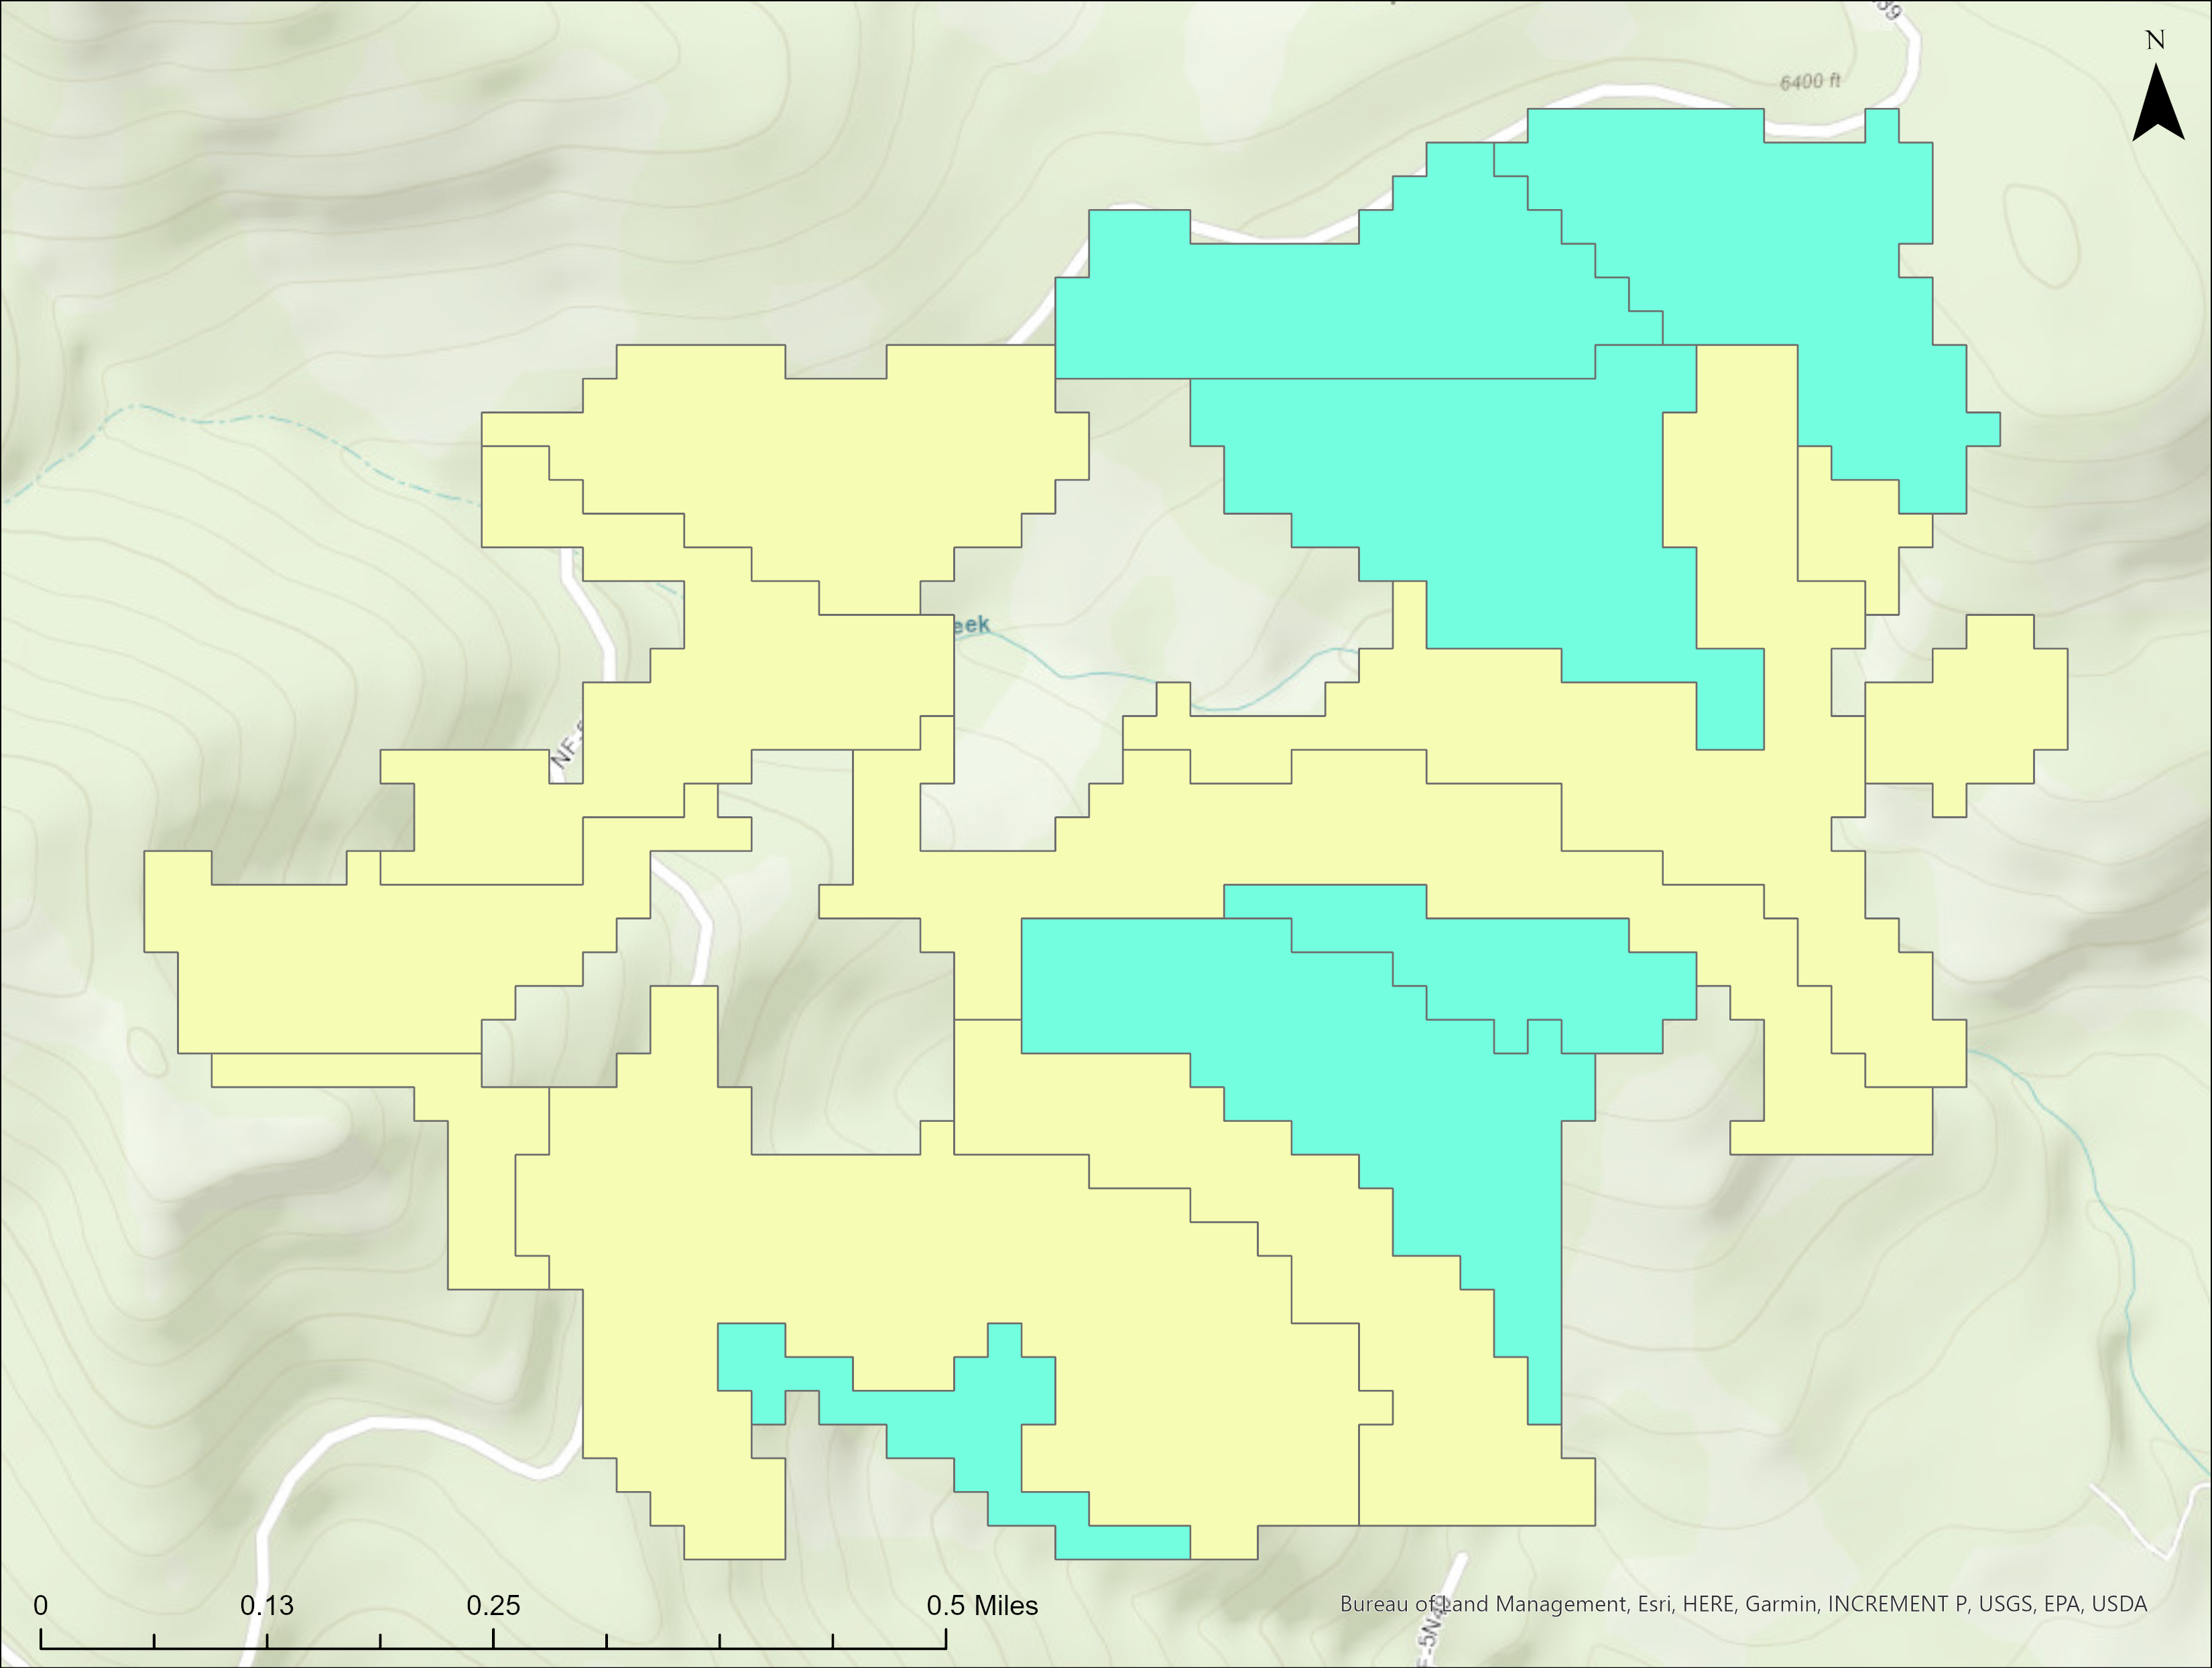
\includegraphics[width=\textwidth]{map1.png}
\end{center}



\newpage
\begin{pbox}[2]
     Based on the greedy heuristic discussed in class, implement your own (better?) version of greedy for this problem. Report the objective value of the solution and visualize the chosen units using the corresponding ArcGIS data layer.
\end{pbox}

We will implement a Bang/Buck greedy heuristic, selecting units in order of benefit-to-area ratio, labeled ``B/B'' in the table below.

\begin{center}
    \begin{tabular}{r|r|r|r|r}
        LMU\_ID & res\_d\_SPM & Acres  & B/B   & Total   \\
        \hline
        37511  & 15.494    & 2.669  & 5.806 & 2.669   \\
        36964  & 26.055    & 8.229  & 3.166 & 10.897  \\
        38060  & 20.605    & 6.894  & 2.989 & 17.792  \\
        35564  & 14.164    & 5.337  & 2.654 & 23.129  \\
        36969  & 11.866    & 5.337  & 2.223 & 28.467  \\
        37507  & 25.308    & 18.014 & 1.405 & 46.481  \\
        37508  & 26.750    & 20.460 & 1.307 & 66.941  \\
        37509  & 26.597    & 23.351 & 1.139 & 90.292  \\
        38061  & 20.639    & 19.793 & 1.043 & 110.085 \\
        37505  & 22.384    & 22.684 & 0.987 &         \\
        38062  & 16.760    & 19.348 & 0.866 &         \\
        36492  & 20.045    & 27.355 & 0.733 &         \\
        37510  & 14.515    & 20.238 & 0.717 &         \\
        36494  & 10.572    & 15.790 & 0.670 &         \\
        38063  & 16.727    & 30.690 & 0.545 &         \\
        36493  & 18.750    & 48.927 & 0.383 &        
        \end{tabular}
\end{center}

Selecting units in order of B/B, while remaining under the capacity threshold, we take the first eight units. While this selection is still short of the capacity threshold, there are no remaining units whose area is less than the remaining capacity, so we can select no more units. Hence, we select the units
\[
    37511, 36964, 38060, 35564, 36969, 37507, 37508, 37509,
\]
giving us a total area of $90.292$. Summing over the benefit of the selected units gives us an objective value of $166.839$, higher than the previous heuristic technique.

\begin{center}
    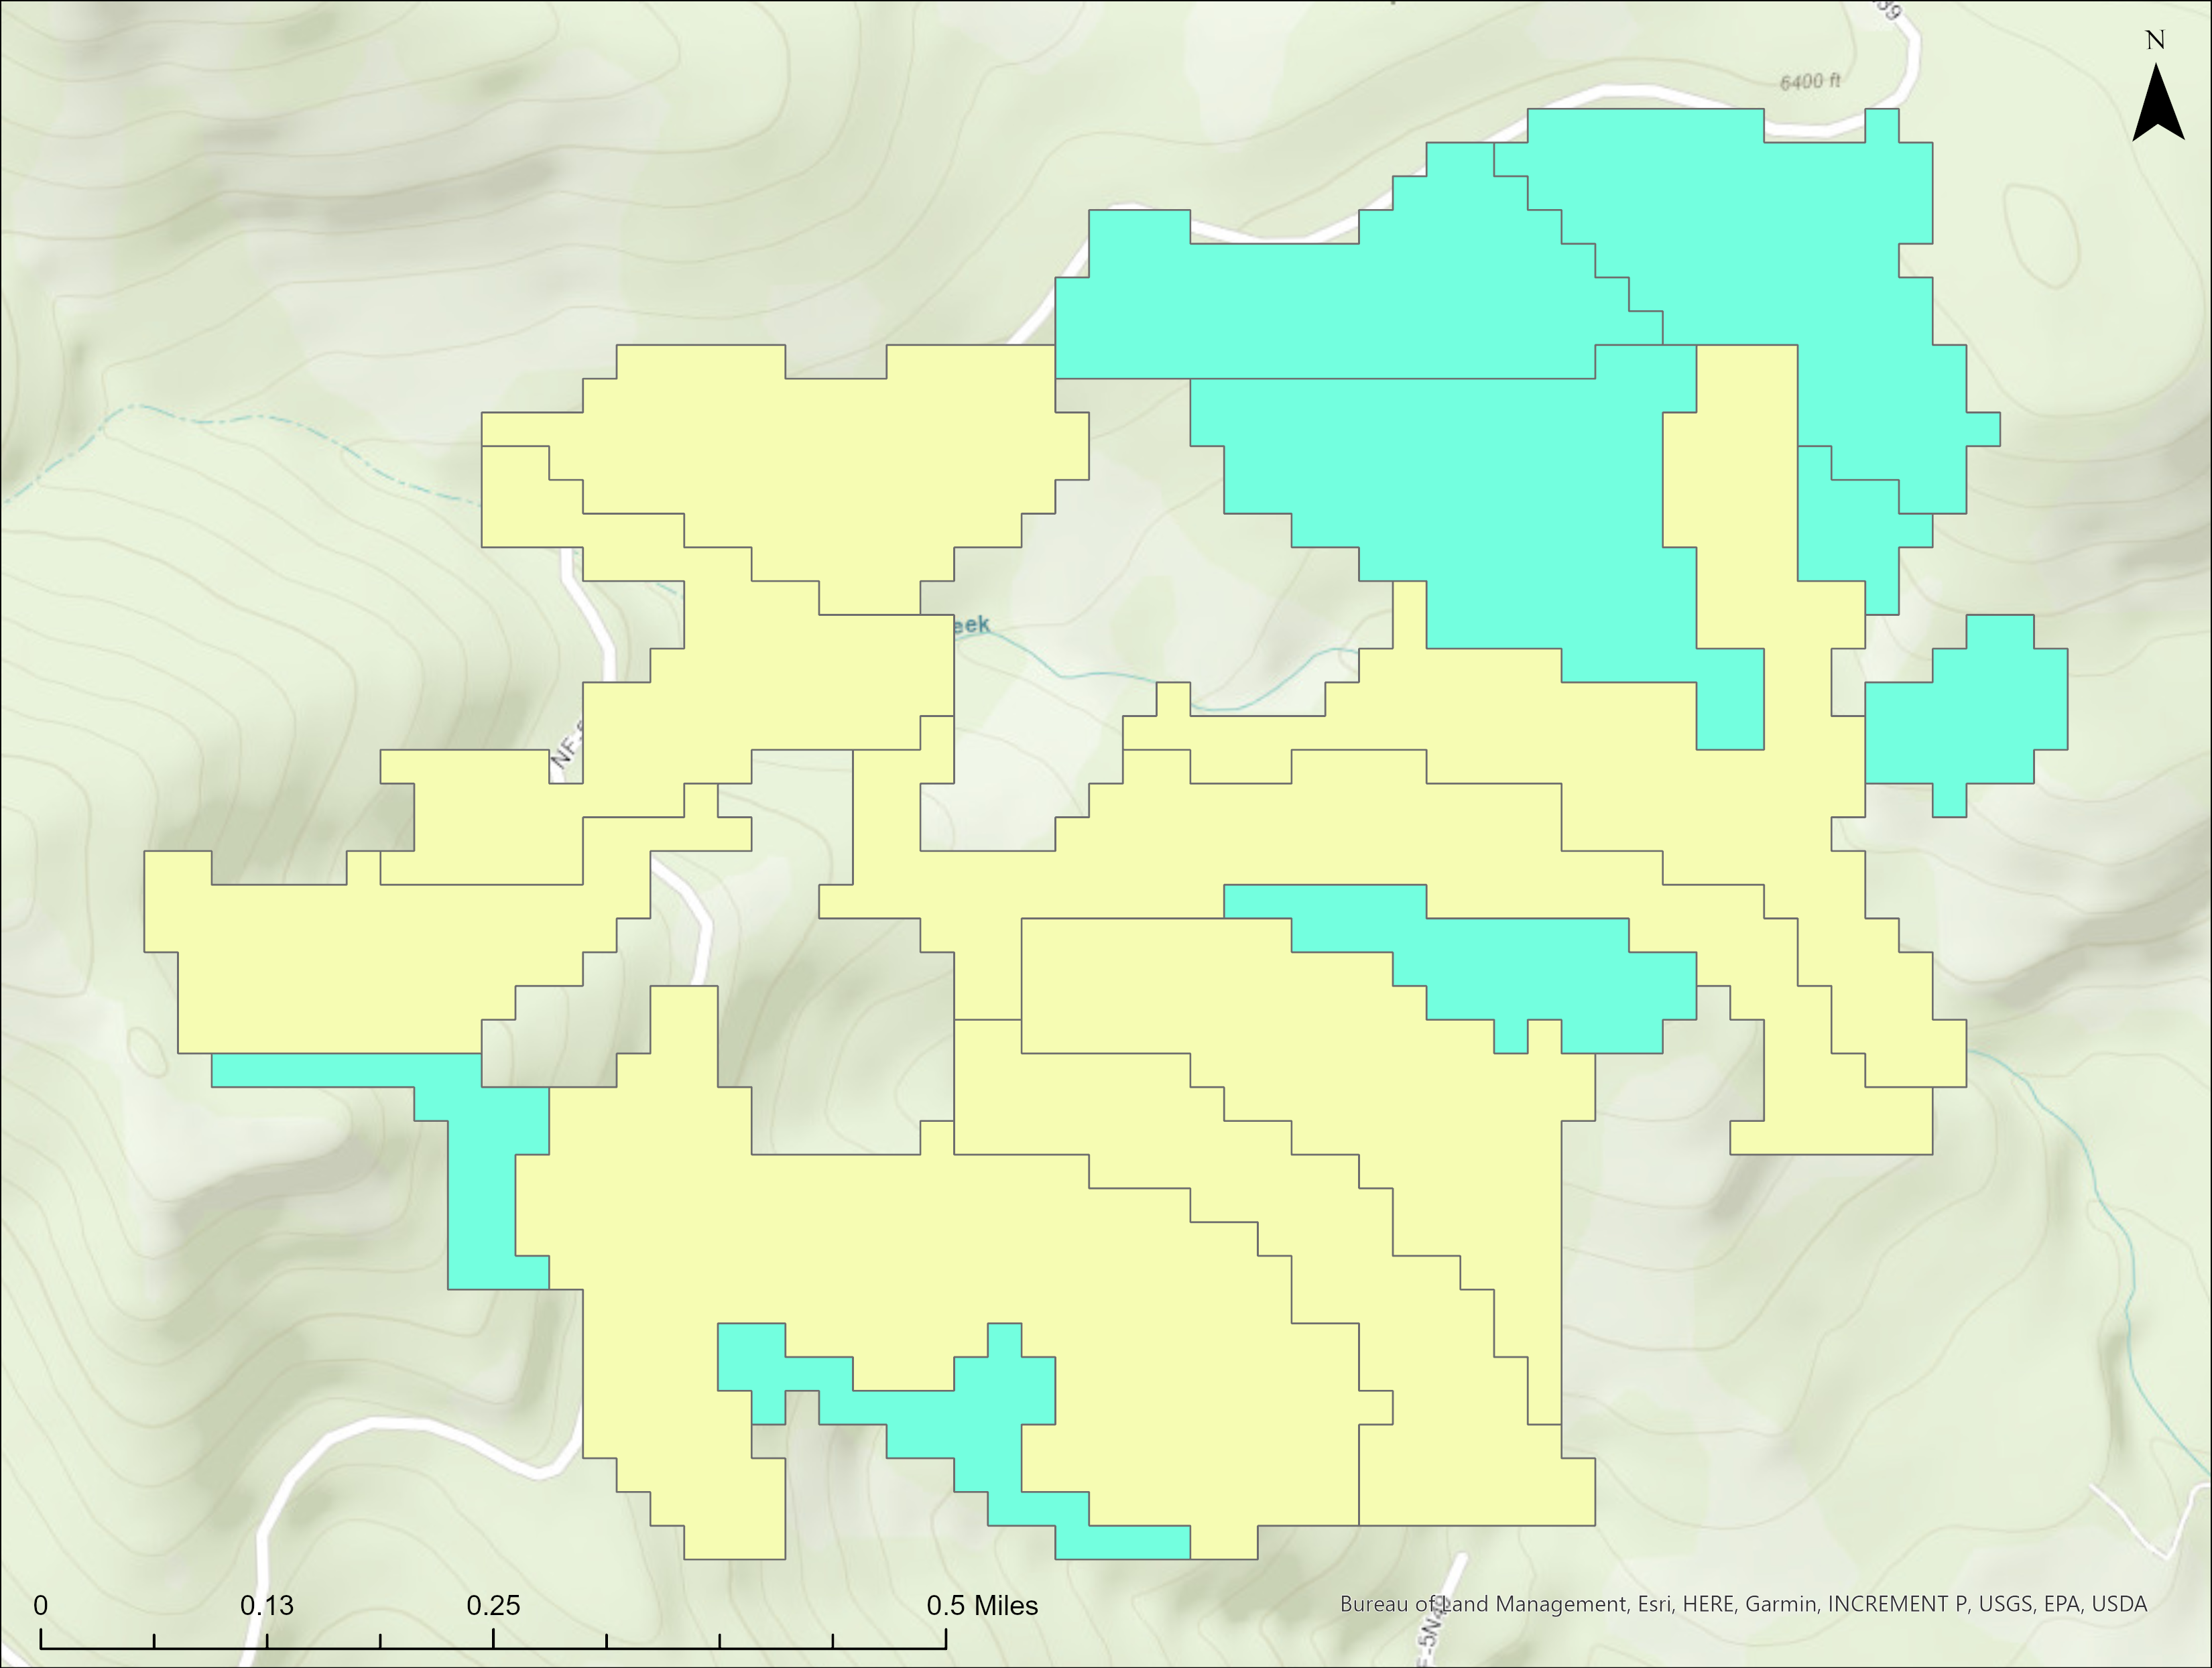
\includegraphics[width=\textwidth]{map2.png}
\end{center}





\newpage
\begin{pbox}[3]
     Solve the problem as a linear program (no integer requirements). Report the solution and solver details and visualize the chosen units using the corresponding ArcGIS data layer. In a short paragraph, discuss whether the solution makes sense for planning and management decision making. Include the Xpress code that you developed and/or modified.
\end{pbox}

\begin{center}
    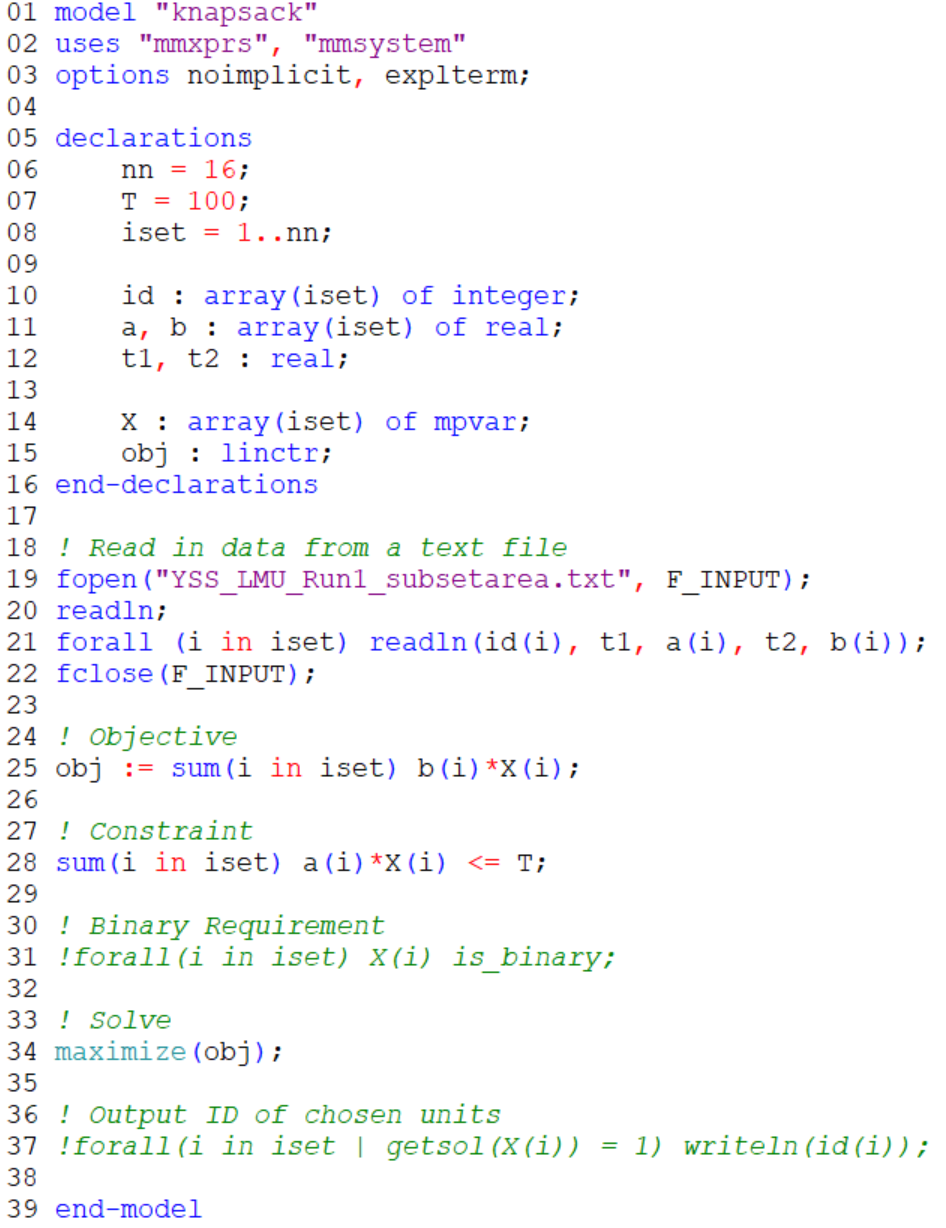
\includegraphics[width=0.6\textwidth]{code1.png}
\end{center}

The linear program was solved by Xpress using the simplex dual algorithm and a produced an optimal solution with an objective value of $580.568$, much higher than either of the heuristic solutions. However, looking at the decision variable values, all are zero except for $X(12) = 37.271$, which corresponds to unit $37511$. In the original interpretation for the decision variables, unit $i$ should be selected if $x_i = 1$ and should not be if $x_i = 0$. We have no useful direct interpretation for other values. The interpretation which is closest to reality is to only select unit $37511$.

\begin{center}
    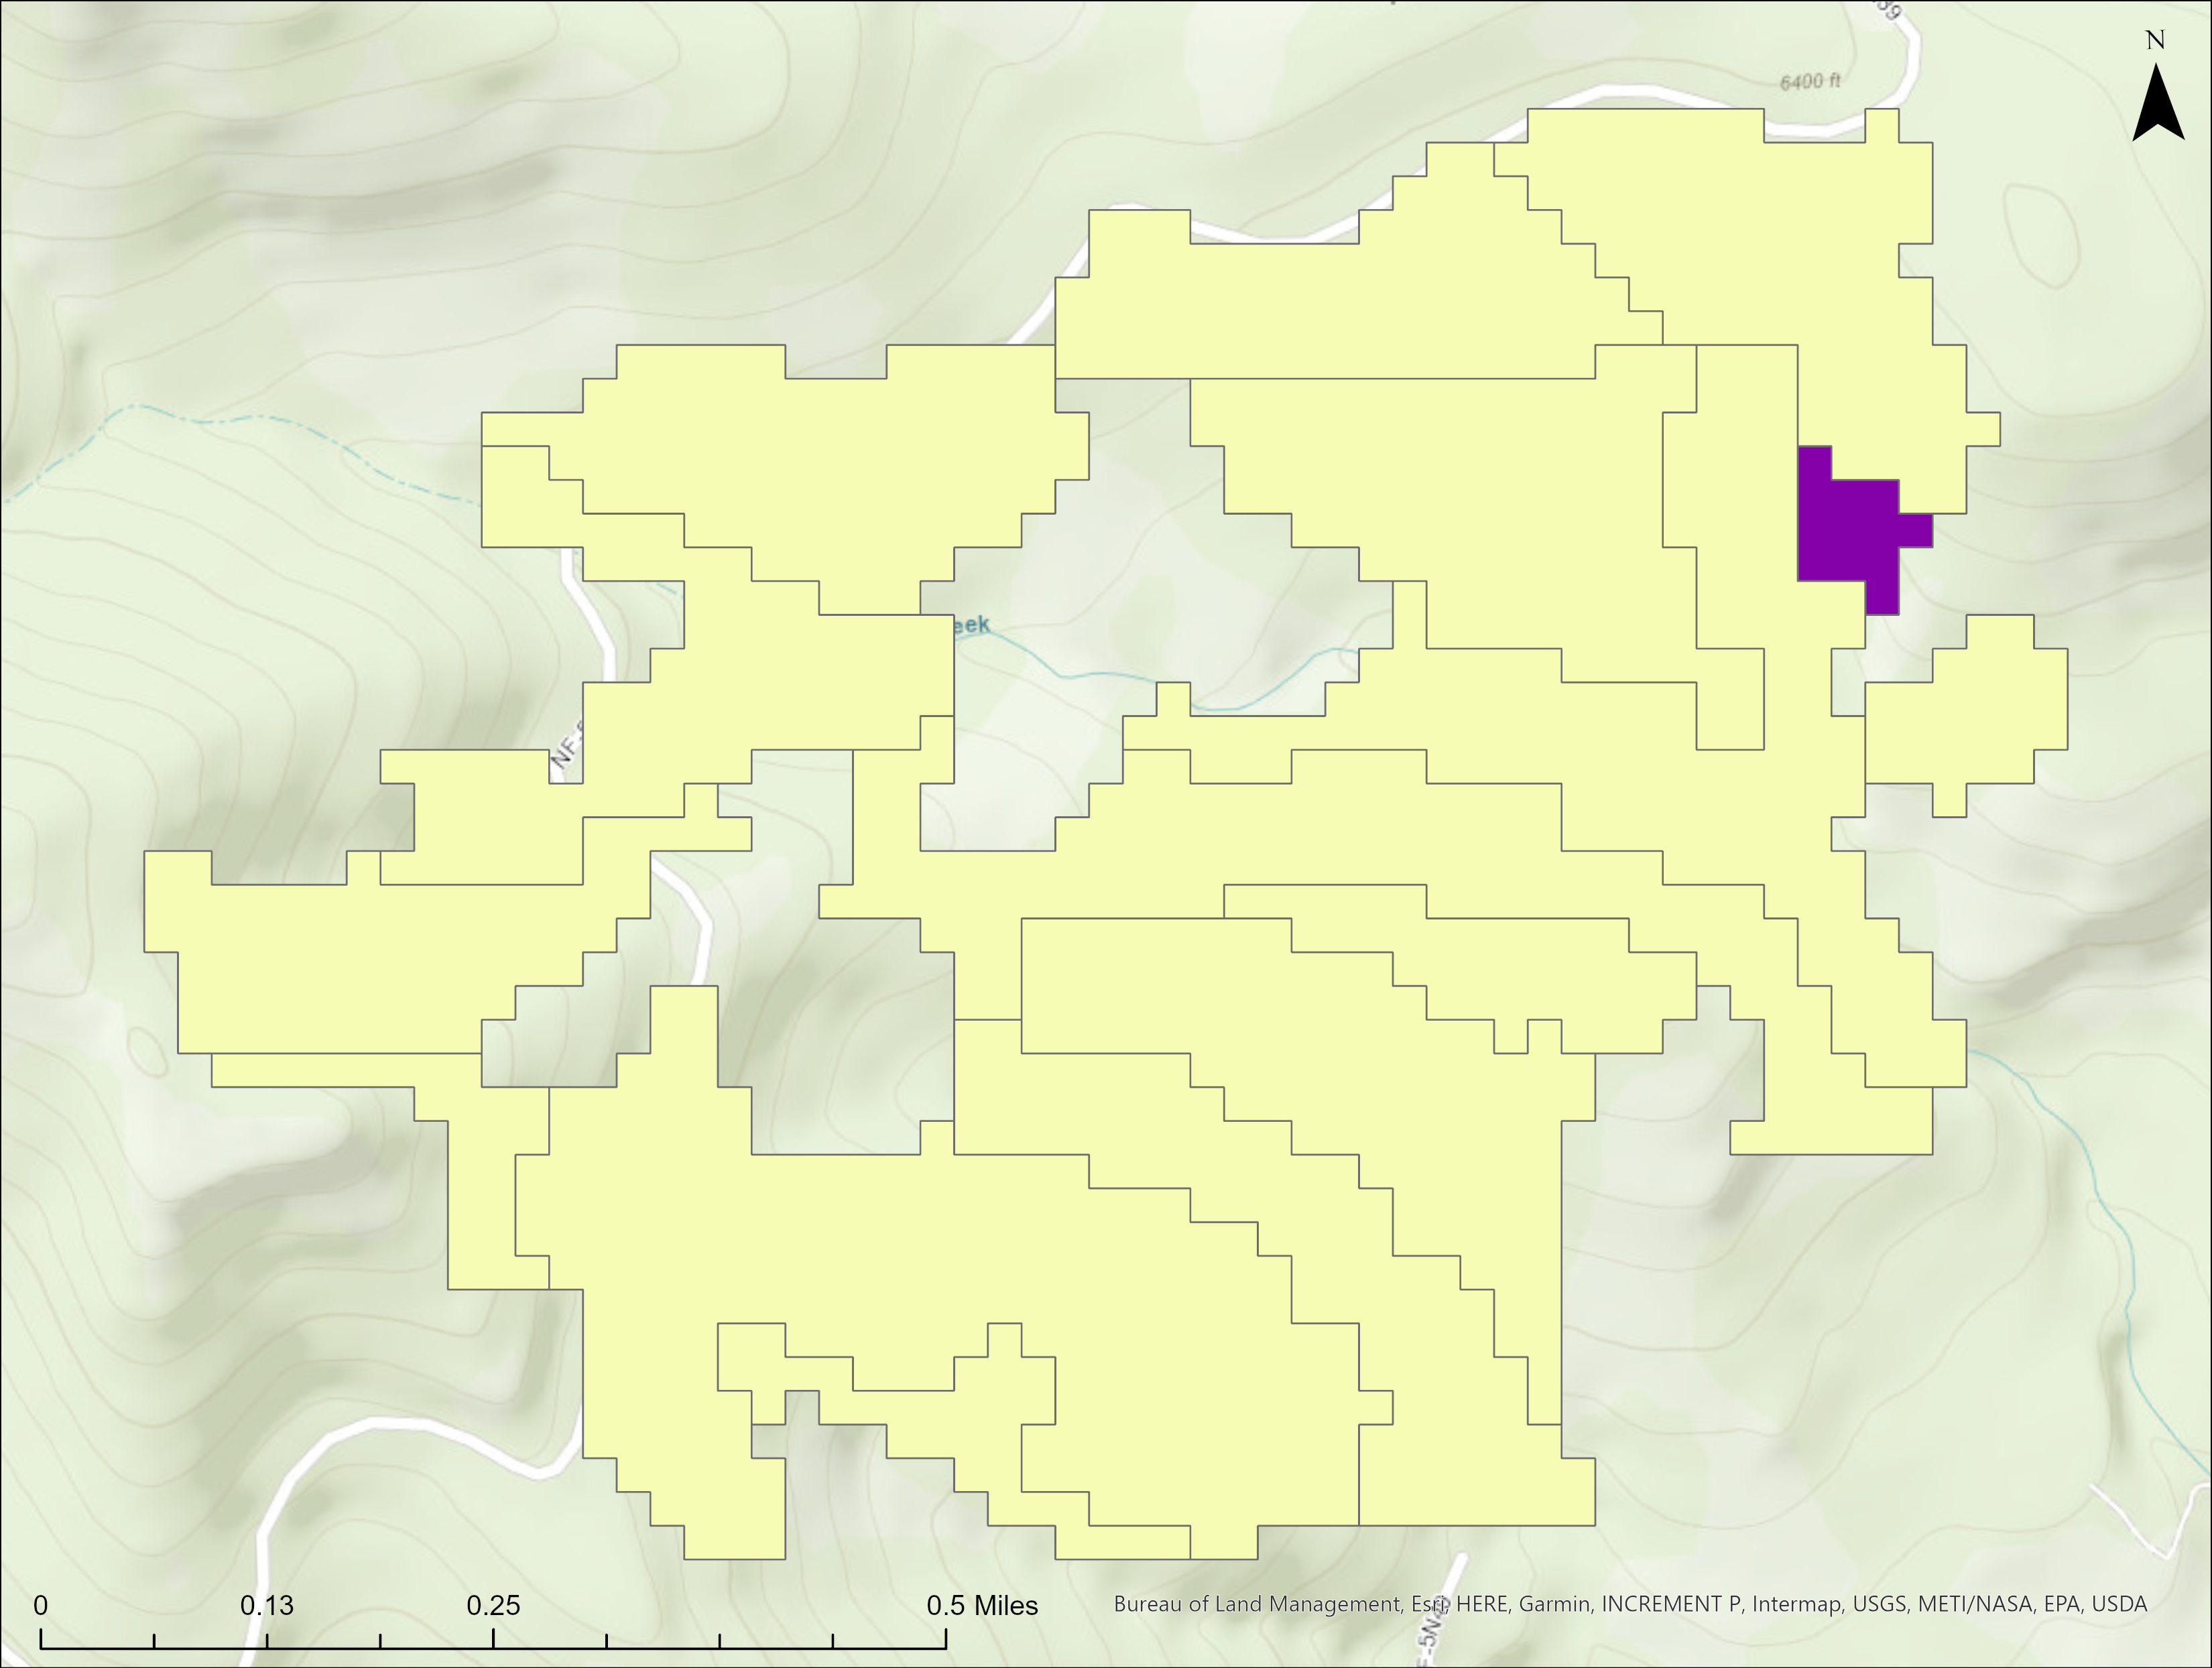
\includegraphics[width=\textwidth]{map3.png}
\end{center}




\newpage
\begin{pbox}[4]
     Solve the problem as an integer program. Report the solution and solver details and visualize the chosen units using the corresponding ArcGIS data layer. In a short paragraph, discuss whether the solution makes sense for planning and management decision making. Include the Xpress code that you developed and/or modified.
\end{pbox}

\begin{center}
    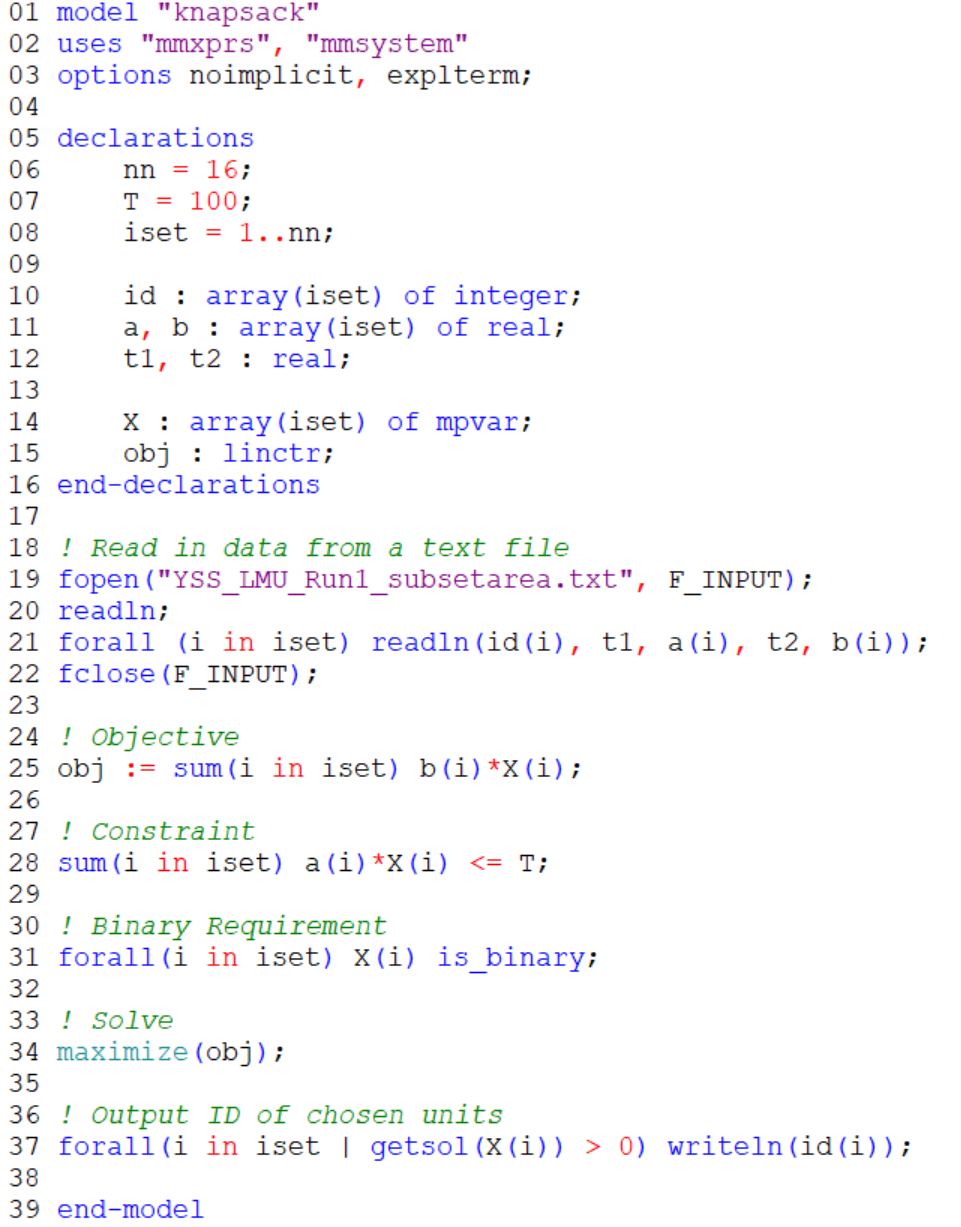
\includegraphics[width=0.6\textwidth]{code2.png}
\end{center}

The binary linear program was solved by Xpress using a combination of the simplex dual algorithm and a global integer search, producing an optimal solution with an objective value of $166.839$, the same as the modified greedy heuristic solution objective in Section 2. In fact, the selected units are
\[
    37511, 36964, 38060, 35564, 36969, 37507, 37508, 37509,
\]
which are precisely the same units selected as in Section 2. As before, selecting these units will give a total area of $90.292$. And since Xpress indicated that the solution was optimal, then we know that there is no better selection of units which remains under the capacity threshold.

\begin{center}
    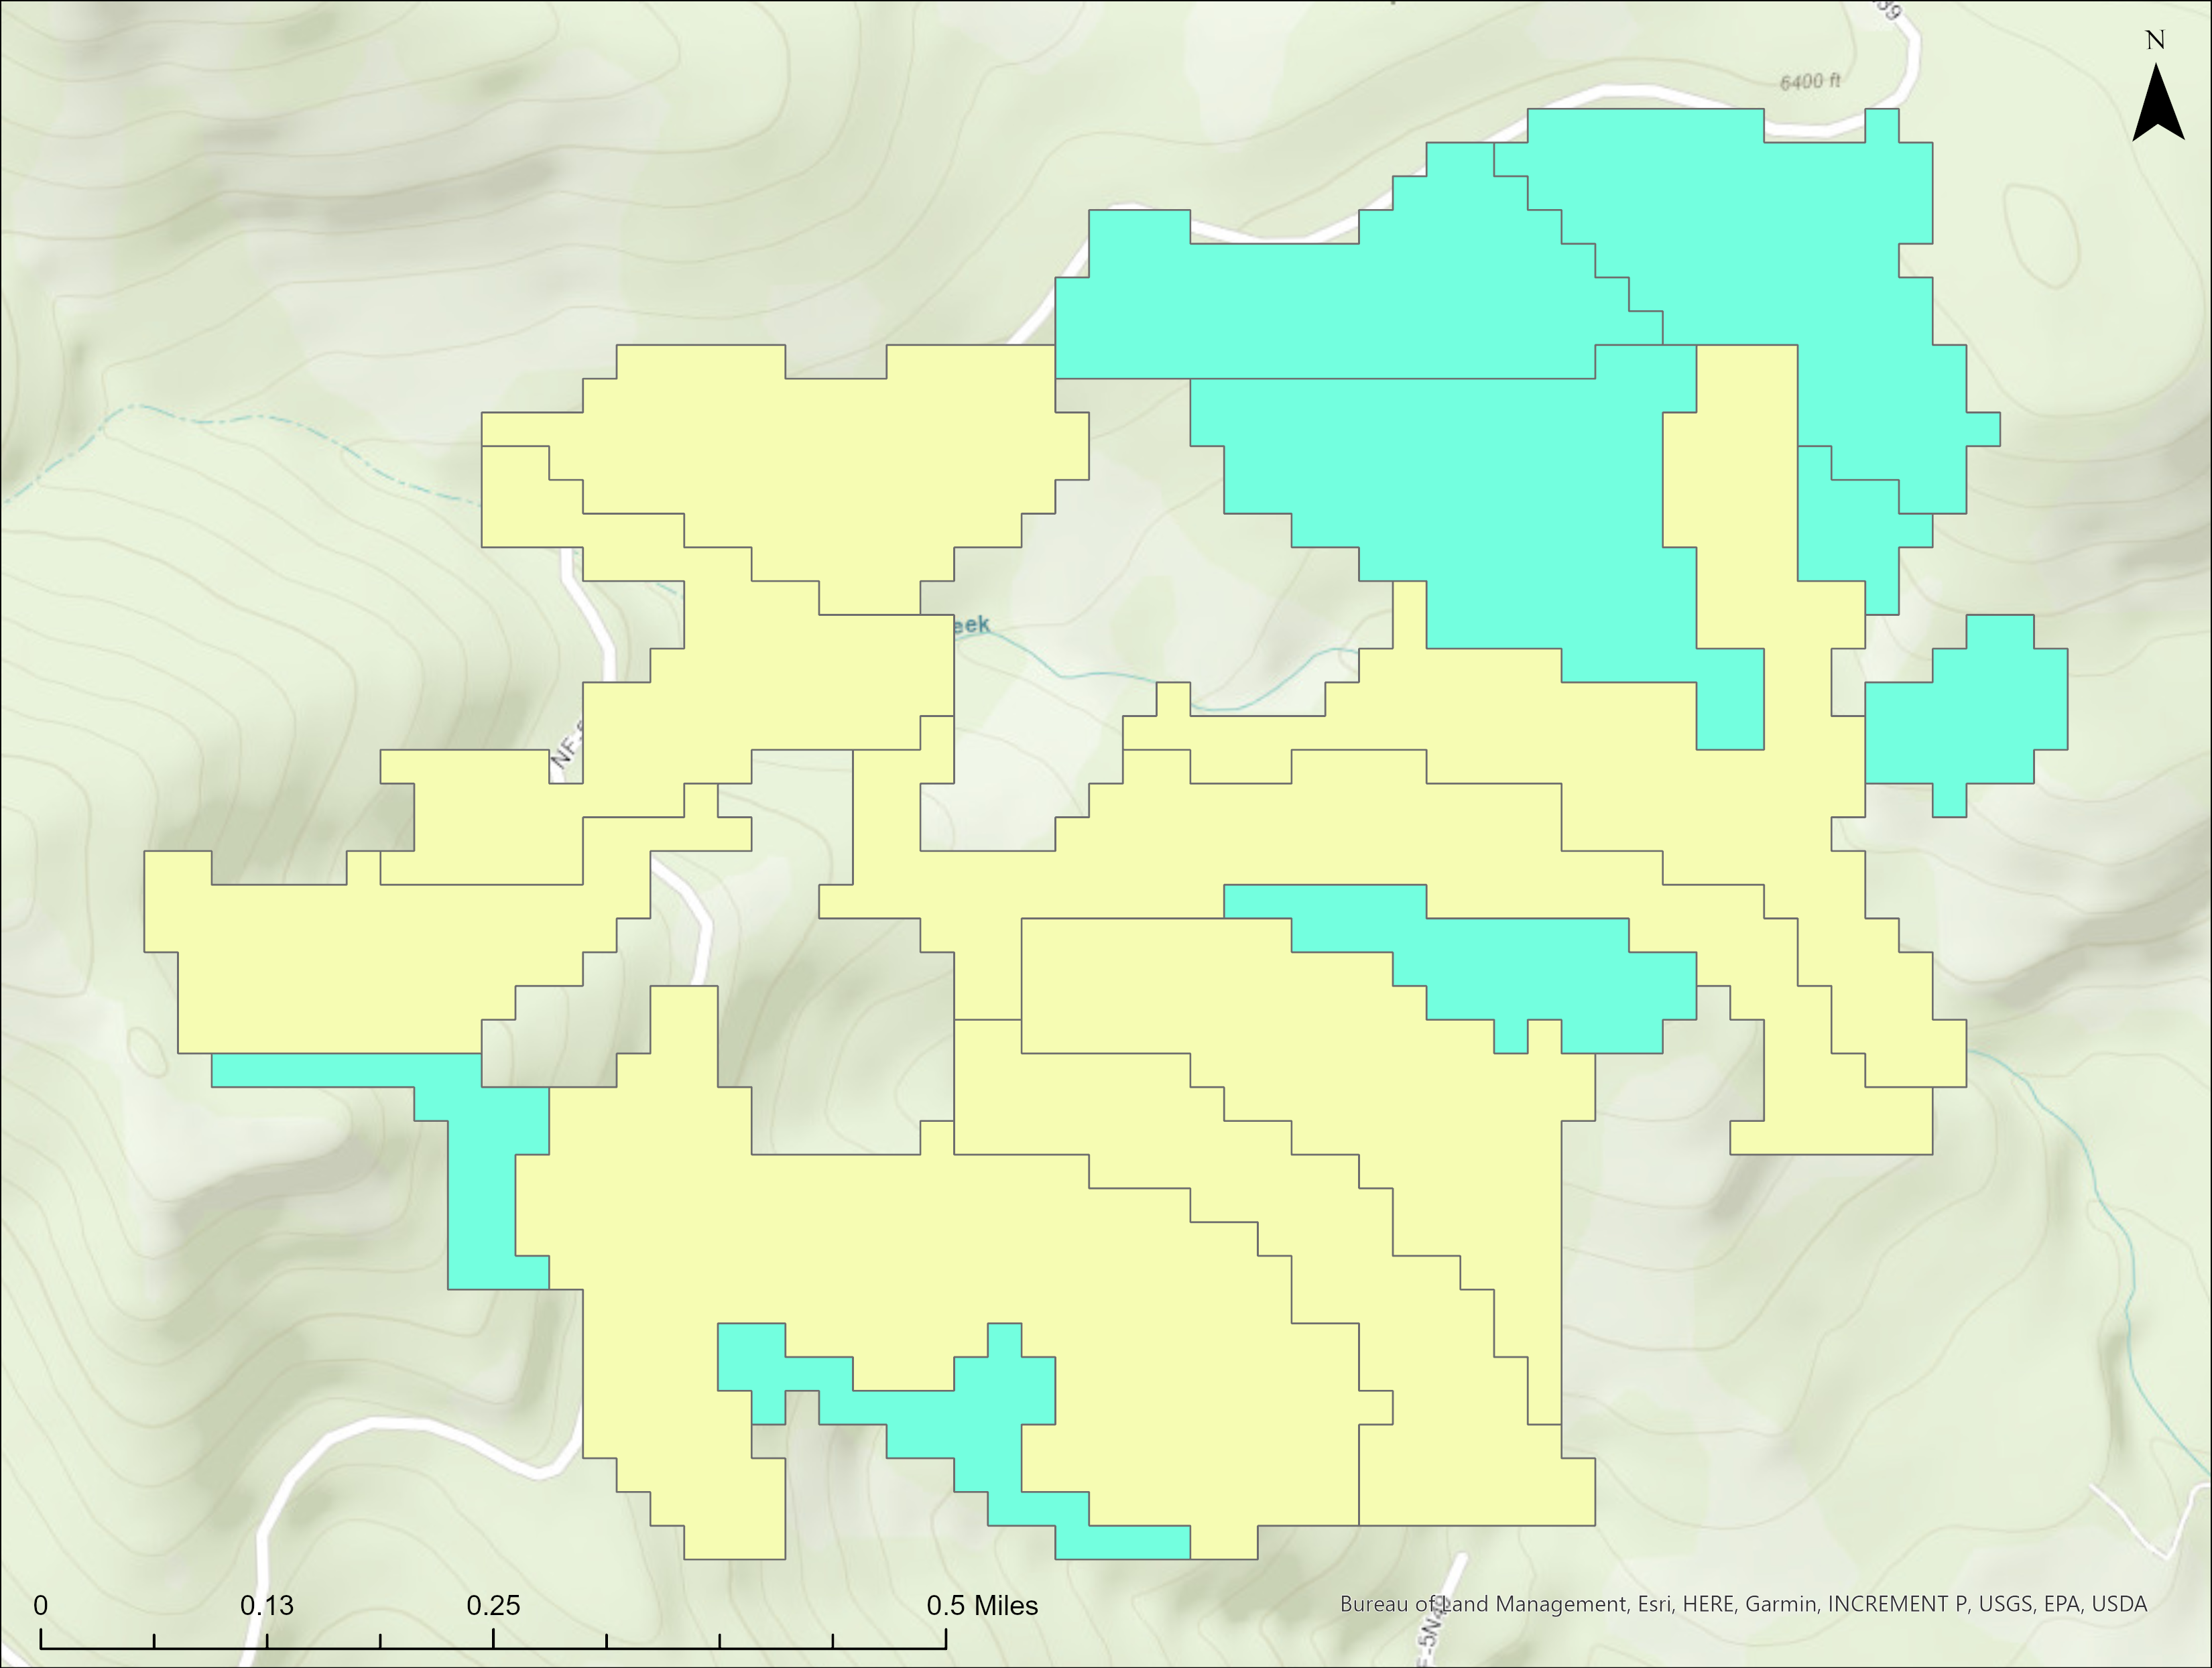
\includegraphics[width=\textwidth]{map2.png}
\end{center}




\begin{pbox}[5]
     In a paragraph, compare and contrast your heuristic and Xpress solutions.
\end{pbox}

The original greedy heuristic considered only the benefit contribution of each unit, and not the area. On the other hand, the modified greedy heuristic prioritized efficiency of benefit with respect to area, by selecting based on the benefit-to-area ratio. Since the latter produced a better solution, we can therefore conclude that the benefit-to-area ratio is a more meaningful metric by which to prioritize units. Moreover, the modified greedy heuristic and the integer Xpress model produced the same solution, so we know it to be an optimal solution. So the benefit-to-area ratio appears to be a sufficiently meaningful metric by which to rank units, as no other metric would produce a better solution. It may be the case that with a larger, but similar, data set would have optimal solutions which could not be found by a simple greedy heuristic. But the results here provide evidence that it is an effective heuristic for selecting units, if advanced solving software is not available.

\end{document}